\documentclass[14pt]{extarticle}
\usepackage[a4paper,
            left=3cm,
            right=1.5cm,
            top=2cm,
            bottom=2cm,
            includehead,includefoot,headheight=0pt,%showframe,
            nohead, nofoot, nomarginpar, 
            ]{geometry}
\linespread{1.5}
\usepackage{silence}
\WarningsOff[fancyhdr]
\usepackage{fancyhdr}
\usepackage{setspace}
\usepackage{listings}
\usepackage{booktabs}
\usepackage{siunitx}
\usepackage[utf8]{inputenc}
\usepackage[T1,T2A]{fontenc}
\usepackage[english, russian]{babel}
\usepackage{amsmath,mathtools,amssymb}
\fontsize{14}{17.3}\selectfont
\usepackage[table,dvipsnames]{xcolor}
\usepackage{soulutf8}
\usepackage{multirow}
\definecolor{LightGray}{rgb}{0.95,0.95,0.95}
\newcommand\college{Томский техникум информационных технологий}
%%%%%%%%%%%%%%%%%%%%%%%%%%%%%%%%%%%%%%%%%%%%%%%%%%%%%%%%%%%%%%%%%%%%%%%%%%%%%%%%
\definecolor{codegreen}{rgb}{0,0.6,0}
\definecolor{codegray}{rgb}{0.5,0.5,0.5}
\definecolor{codepurple}{rgb}{0.18,0,0.82}
\definecolor{backcolour}{rgb}{0.95,0.95,0.92}
\lstdefinestyle{mystyle}{
	backgroundcolor=\color{backcolour},
	commentstyle=\color{codegreen},
	keywordstyle=\color{codepurple},
	numberstyle=\tiny\color{codegray},
	stringstyle=\color{codepurple},
	basicstyle=\ttfamily\footnotesize,
	breakatwhitespace=false,
	breaklines=true,
	captionpos=b,
	keepspaces=true,
	numbers=left,
	numbersep=5pt,
	showspaces=false,
	showstringspaces=false,
	showtabs=false,
	tabsize=2,
	numbers=none,
	framesep=10pt,
	xleftmargin=7pt,
	xrightmargin=7pt,
	framexleftmargin=7pt,
	framexrightmargin=7pt
}
\lstset{style=mystyle}

\usepackage{enumitem}

\usepackage{listings}

\setlength\parindent{1.25cm}
\setlength{\footskip}{30pt}
\usepackage{indentfirst}

%\counterwithin{figure}{chapter}
%\counterwithin{table}{chapter}

\usepackage{titlesec}
\titleformat{\section}{\normalfont\normalsize\filcenter}{\thesection}{0.3em}{}
\titleformat{\subsection}{\normalfont\normalsize}{\thesubsection}{0.3em}{}
\titleformat{\subsubsection}{\normalfont\normalsize}{\thesubsubsection}{0.3em}{}

\titlespacing*{\section}{0pt}{0pt}{20pt}
\titlespacing*{\subsection}{1.25cm}{0pt}{20pt}
\titlespacing*{\subsubsection}{1.25cm}{0pt}{20pt}

\newlist{mylist}{itemize}{1}
\setlist[mylist]{label=—, leftmargin=1.9, rightmargin=0pt}

\newlist{listNoSpaceAfter}{enumerate}{1}
\setlist[listNoSpaceAfter]{label=\arabic*), leftmargin=0cm, itemindent=1.9cm, noitemsep, before=\vspace{-16px}, after=\vspace{-20px}}

\setlist[enumerate]{label=\arabic*), leftmargin=0cm, itemindent=1.9cm, noitemsep, before=\vspace{-16px}, after=\vspace{-12px}}

\usepackage{fontspec}
\setmainfont{pt-astra-serif-regular.ttf}

\usepackage{unicode-math}
\defaultfontfeatures[pt-astra-serif-regular]
    { %Path = {/},
      Extension = .ttf }

\babelfont{tt}{Cousine}

\makeatletter
\renewcommand*\normalsize{%
  \@setfontsize\normalsize{14}{21}
}
\makeatother

\usepackage{caption}
\DeclareCaptionLabelSeparator{emdash}{\space\textemdash\space}
\captionsetup[figure]{name={Рисунок}, labelsep=endash}
\captionsetup[table]{name={Таблица}, labelsep=endash}
\captionsetup[listing]{name={Листинг}, labelsep=endash}
\captionsetup[table]{skip=0pt, singlelinecheck=off}

\usepackage{caption}
\usepackage[newfloat]{minted}
\usepackage{ragged2e}
\captionsetup[lstlisting]{position=top, labelsep=endash, justification=justified, singlelinecheck=off}

\fancyhfoffset[E,O]{0pt}

\setlength{\belowdisplayskip}{0pt} \setlength{\belowdisplayshortskip}{0pt}
\setlength{\abovedisplayskip}{0pt} \setlength{\abovedisplayshortskip}{0pt}

\newcommand\variant[1]{#1}
\newcommand\answer[2]{#2}
\newcommand\Group{600}
\newcommand\FirstStudent{И.\,И. Иванов}
%\newcommand\SecondStudent{П.\,П. Петров}
\newcommand\Type{Отчёт о лабораторно-практической работе №\,2}
\newcommand\Topic{Решение уравнений}

\begin{document}
\pagestyle{fancy}
\chead{}
\cfoot{}
\lhead{}
\rhead{}
\renewcommand{\headrulewidth}{0pt}
\renewcommand{\footrulewidth}{0pt}
\cfoot{\thepage}
\thispagestyle{empty}

\setmathfont[range=up/{num}]{pt-astra-serif-regular.ttf}
\setmathfont[range=it/{latin,Latin}]{pt-astra-serif-italic.ttf}


\begin{spacing}{1.5}
\begin{center}
ДЕПАРТАМЕНТ ОБРАЗОВАНИЯ ТОМСКОЙ ОБЛАСТИ\vspace{0px}

ОБЛАСТНОЕ ГОСУДАРСТВЕННОЕ БЮДЖЕТНОЕ\vspace{-10px}\\ 
ПРОФЕССИОНАЛЬНОЕ ОБРАЗОВАТЕЛЬНОЕ УЧРЕЖДЕНИЕ\vspace{-10px}\\
\raisebox{.14ex}{«}ТОМСКИЙ ТЕХНИКУМ ИНФОРМАЦИОННЫХ ТЕХНОЛОГИЙ\raisebox{.14ex}{»}

\vspace{0.5cm}

Специальность 09.02.07 Информационные системы и программирование

\vspace{4cm}

\Type\vspace{-10px}\\по дисциплине «Численные методы»

\MakeUppercase{\Topic}

\end{center}


\vspace{3cm}

Студент\ifdefined\SecondStudent ы \fi~гр. \Group\vspace{-5px}

«\rule{5mm}{0.15mm}» \rule{20mm}{0.15mm} \the\year~г.
\hspace{16mm} \rule{35mm}{0.15mm}
\hspace{2mm} \FirstStudent

\ifdefined\SecondStudent

«\rule{5mm}{0.15mm}» \rule{20mm}{0.15mm} \the\year~г.
\hspace{16mm} \rule{35mm}{0.15mm}
\hspace{2mm} \SecondStudent

\fi

\vspace{-10px}

Преподаватель\vspace{-5px}

«\rule{0.5cm}{0.15mm}» \rule{2cm}{0.15mm} \the\year~г.
\hspace{16mm} \rule{35mm}{0.15mm}
\hspace{2mm} Д.\,И. Жабин


\vspace{2cm}

\begin{center}
Томск \the\year{}
\end{center}
\newpage
\end{spacing}

\cfoot{\thepage}

\section{\MakeUppercase{Постановка задачи}}

В ходе выполнения лабораторно-практической работы требуется составить уравнение для решения указанной в~варианте задачи, написать и отладить программу, реализующую указанные методы, и проверить полученный результат.

Вариант №\,16. $x^2 - 34 = 0$. Решить задачу с~помощью методов дихотомии, хорд и грубой силы (перебора).

\newpage

\section{\MakeUppercase{Ход работы}}

Уравнение: $x^2 - 34 = 0$.

%%%%%%%%%%%%%%%%%%%%%%%%%%%%%%%%%%%%%%%%

\vspace{1.5em}\subsection{Метод дихотомии}

Добавьте описание метода. Код представлен в листинге \ref{listing:dichotomy}.

\vspace{1.5em}
\begin{lstlisting}[
	language=R,
	caption=Код для метода дихотомии,
	label=listing:dichotomy,
        captionpos=tr,
	]
dichotomy <- function(f, a, b, epsilon) {
    repeat {
        x <- (a + b) / 2
        y <- f(x)
        ifelse (f(a) * y < 0, b <- x, a <- x)
        if (abs(y) <= epsilon) {
            break
        }
    }
    x
}
\end{lstlisting}

%%%%%%%%%%%%%%%%%%%%%%%%%%%%%%%%%%%%%%%%

\subsection{Метод хорд}

Добавьте описание метода. Код представлен в листинге \ref{listing:chordes}.

\vspace{1.5em}
\begin{lstlisting}[
	language=R,
	caption=Код для метода хорд,
	label=listing:chordes,
        captionpos=tr,
	]
Your code goes here.
\end{lstlisting}

%%%%%%%%%%%%%%%%%%%%%%%%%%%%%%%%%%%%%%%%

\subsection{Метод грубой силы (перебора)}

Добавьте описание метода. Код представлен в листинге \ref{listing:bruteforce}.

\begin{lstlisting}[
	language=R,
	caption=Код для метода грубой силы (перебора),
	label=listing:bruteforce,
        captionpos=tr,
	]
Your code goes here.
\end{lstlisting}

Выходные данные полученной программы представлены в таблице \ref{tab:results}.

\begin{table}[!h]
	\sisetup{output-decimal-marker={,}}
	\centering
	\caption{Результаты запуска программы}
	\label{tab:results}
	\begin{tabular}{|l|S|}
		\specialrule{.4pt}{2pt}{0pt}
		Метод                        & Решение   \\
		\specialrule{.4pt}{0pt}{0pt}
		Метод грубой силы (перебора) & 1,44      \\
		Метод хорд                   & 1,4       \\
		Метод Ньютона (касательных)  & 1,44      \\
		\specialrule{.8pt}{0pt}{2pt}
	\end{tabular}
\end{table}

Из рисунка \ref{fig:plot} видно, что график функции пересекает ось абсцисс примерно там же.

\begin{figure}[!h]
	\centering
	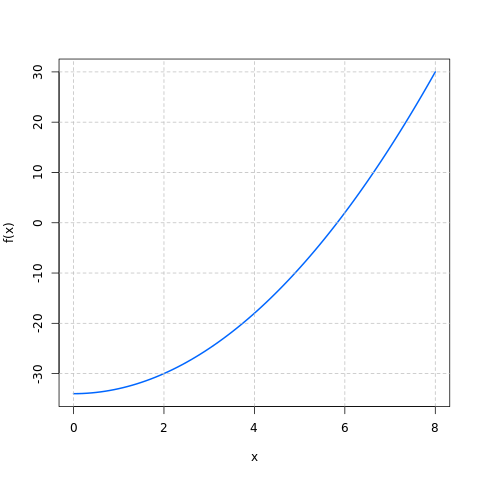
\includegraphics[width=0.75\textwidth]{plot.png}
	\caption{Графическое решение}
	\label{fig:plot}
\end{figure}

%%%%%%%%%%%%%%%%%%%%%%%%%%%%%%%%%%%%%%%%

\clearpage

\section{\MakeUppercase{Заключение}}

В ходе выполнения лабораторно-практической работы мы сначала составили уравнение для решения задачи, затем написали и отладили программу, реализующую методы дихотомии, хорд и грубой силы (перебора), и проверили полученный результат.

\end{document}
